\chapter{Autoencoder}
\label{appendix:A}
This appendix gives further information on the autoencoder architecture presented in Chapter \ref{ch:autoencoder_network}.

\section{Pre-Trained VGG Networks}
\label{A:sec:pretrained_autoencoders_from_different_frameworks}
Section \ref{sec:encoder} explained why one wants to leave the encoder with its pre-trained weights fixed in the autoencoder network. 

Nevertheless, it does make a difference how the VGG-19 was trained on the object recognition task. This work uses the pre-trained model from the Caffe framework \cite{caffe} that has the best feature responses. The pre-trained VGG-19 model of the PyTorch framework \cite{PyTorch} seems to be trained for less epochs and therefore does not yield the same quality of feature responses.

The quality of the feature responses directly correlates with the image quality that can be reached. Especially, the strength of checkerboard artifacts seems to be correlated negatively with the quality of the feature responses.

\section{Loss Balancing}
\label{A:sec:balancing_of_feature_loss_and_per_pixel_loss}
The main complexity in training the decoder network with a fixed encoder network is to balance the three presented losses in a way that prevents strong checkerboard artifacts from evolving. 
\begin{align}
\mathcal{L}
= 
\lambda_{\mathrm{pp}}
\cdot
\mathcal{L}_{\mathrm{pp}} +
\lambda_{\mathrm{feat}}
\cdot
\mathcal{L}_{\mathrm{feat}} +
\lambda_{\mathrm{TV}}
\cdot
\mathcal{L}_{\mathrm{TV}}
\end{align}

Using only a per-pixel loss with $\lambda_{\mathrm{pp}} = 1, \lambda_{\mathrm{feat}}=0, \lambda_{\mathrm{TV}}=0$ results in images that are equal to the input image in color and spatial structure. However, the images are in contrast to the ground truth images very blurry and do not reflect fine structures from the input images. This is due to the fact that no high-level features of the images are matched but only the pixel values. Using a $L_1$ loss instead of a $L_2$ loss does not bring any improvement. 

If one combines the per-pixel loss with a feature-loss and the balancing factors $\lambda_{\mathrm{pp}} = 1, \lambda_{\mathrm{feat}}=1, \lambda_{\mathrm{TV}}=0$, almost every image has very strong checkerboard artifacts. This is attributed to not training the encoder. Matching high level features and not training the encoder leads to checkerboard artifacts since the features may not represent the whole information needed to reconstruct an image. 

Therefore, the key idea is to balance $\lambda_{\mathrm{pp}}$ and $\lambda_{\mathrm{feat}}$ in a way to get the best possible tradeoff between visually clear images and no checkerboard artifacts. Figure \ref{fig:A_autoencoder_balancing} shows the balancing process for several factors. Since the images with $\lambda_{\mathrm{pp}} = 25$ and $\lambda_{\mathrm{feat}}=1$ are perceptually most appealing, the autoencoder with those factors is used in this work.
% figure
\begin{figure}[!ht]
  	\includegraphics[width=\textwidth]{img/A_EncoderDecoder_balancing/A.jpeg}
  	\includegraphics[width=\textwidth]{img/A_EncoderDecoder_balancing/B.jpeg}
  	\includegraphics[width=\textwidth]{img/A_EncoderDecoder_balancing/ann.pdf}
	\caption{Visualization of different loss factors of $\lambda_{\mathrm{pp}}$ and $\lambda_{\mathrm{feat}}$.}
	\label{fig:A_autoencoder_balancing}
\end{figure}

\subsection{TV Regularizer}
The TV regularizer can reduce checkerboard artifacts that are still visible in some images. Surprisingly, balancing the TV regularizer with a higher factor does not reduce checkerboard artifacts in a better way but instead makes the checkerboard artifacts better visible. 

While a factor of $\lambda_{\mathrm{TV}}=10^{-3}$ results in gray images and a factor of $\lambda_{\mathrm{TV}}=10^{-4}$ shifts the colors, the best results are achieved by a factor of $\lambda_{\mathrm{TV}}=10^{-6}$. Figure \ref{fig:A_autoencoder_balancing_tv} shows some images which make the effect of the TV regularizer visible.
% figure
\begin{figure}[!ht]
  	\includegraphics[width=\textwidth]{img/A_EncoderDecoder_tv/A.jpeg}
  	\includegraphics[width=\textwidth]{img/A_EncoderDecoder_tv/B.jpeg}
  	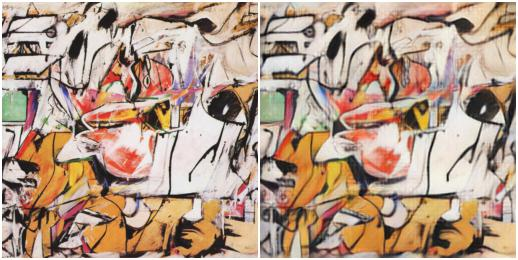
\includegraphics[width=\textwidth]{img/A_EncoderDecoder_tv/C.jpeg}
  	\includegraphics[width=\textwidth]{img/A_EncoderDecoder_tv/ann.pdf}
	\caption{Visualization of different loss factors of $\lambda_{\mathrm{TV}}$.}
	\label{fig:A_autoencoder_balancing_tv}
\end{figure}

